%!TEX root = ../thesis.tex
%*******************************************************************************
%****************************** Fourth Chapter *********************************
%*******************************************************************************
\graphicspath{{Chapter4/Figs/Vector/}{Chapter4/Figs/}}

%%%%%%%%%%%%%%%%%%%%%%%%%%%%%%%%%%%%%%%%%%%%%%%%%%%%%%%%%%%%%%%%%%%%%%%%%%%%%%%%
% Trip Price Calculation System
%%%%%%%%%%%%%%%%%%%%%%%%%%%%%%%%%%%%%%%%%%%%%%%%%%%%%%%%%%%%%%%%%%%%%%%%%%%%%%%%
% - Which logic and information is required to calculate a trip price?
%
\chapter{Trip Price Calculation System}
\section{Introduction}
In the previous chapter, information dependencies were discussed. This chapter clarifies which information should comprise a price breakdown to reflect that of the legacy system, how the system should be structured, what logical flow of information is to be contrived, and how different pieces of information that are stored and processed should restrict the time and space dimensions of a price rule without blurring the straightforwardness of the system.

%%%%%%%%%%%%%%%%%%%%%%%%%%%%%%%%%%%%%%%%%%%%%%%%%%%%%%%%%%%%%%%%%%%%%%%%%%%%%%%%
% Data Model
%%%%%%%%%%%%%%%%%%%%%%%%%%%%%%%%%%%%%%%%%%%%%%%%%%%%%%%%%%%%%%%%%%%%%%%%%%%%%%%%
%
\section{The System}


removev class diagram
\begin{figure}[H]
	\centering
	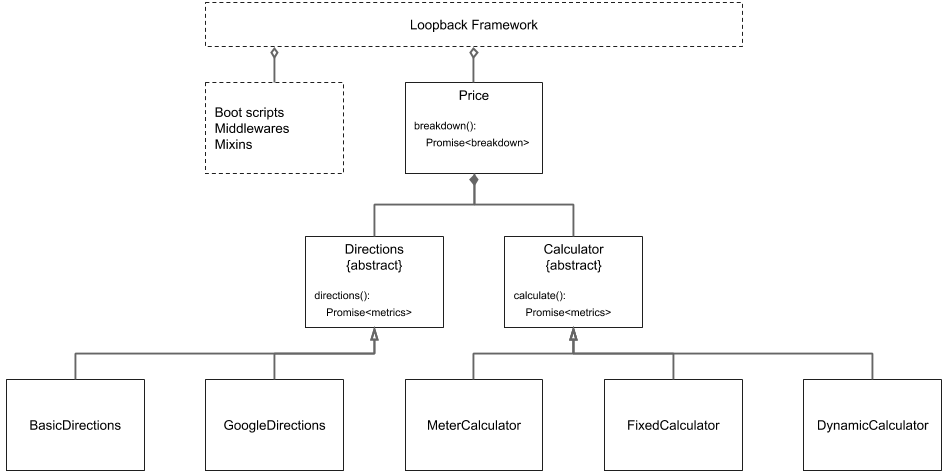
\includegraphics[width=1\textwidth]{ClassDiagram}
	\caption[Class Diagram]{Class diagram.}
	\label{fig:ClassDiagram}
\end{figure}

\mynote{Expand on
	interfaces,
	static strong types,
	type hinting,
	OOP en FP mixen,
	OOP voor grote structuur,
	FP voor solide operaties,
	SOLID,
	Gang of Four,
	Loose coupling high cohesion,
	Async,
	Strategy pattern,
}

The Price object is composed of a Directions and a Calculator Class, both of which expose only one instance method, directions and calculate respectively. The entire class diagram should adhere to Uncle Bob's SOLID principles. State and mutations should be fully encapsulated, leaving only static functions exposed. These functions aim to mutate data in a pure way, meaning that no state is changed outside of the function scope, and that the function is absolutely honest about its parameters and return values. As discussed in the previous chapter, Typescript plays an important role in mixing OOP and FP together. The database schema desgin as shown in the previous chapter gives an inpression on the different pieces of information required to calculate a price. Such a schema provides a good insight in the relationships that different entities have, but may distract from the actual story that is happening within each calculation. In Figure \ref{fig:DataModel} a conceptual model can be seen having association and composition relations in UML notation. This model will be used to refer to throughout this chapter.

\begin{figure}[H]
	\centering
	
\includegraphics[width=1\textwidth]{DataModel}
	\caption[DataModel]{Conceptual data model showing database entity relations.}
	\label{fig:DataModel}
\end{figure}

%%%%%%%%%%%%%%%%%%%%%%%%%%%%%%%%%%%%%%%%%%%%%%%%%%%%%%%%%%%%%%%%%%%%%%%%%%%%%%%%
% Locations
%%%%%%%%%%%%%%%%%%%%%%%%%%%%%%%%%%%%%%%%%%%%%%%%%%%%%%%%%%%%%%%%%%%%%%%%%%%%%%%%
%
\section{Locations}
Locations and timeframes are the big filters that reduce the amount of potential matching rules and discounts based on space and time. The implementation for location queries ...
\mynote{Working on locations}

%%%%%%%%%%%%%%%%%%%%%%%%%%%%%%%%%%%%%%%%%%%%%%%%%%%%%%%%%%%%%%%%%%%%%%%%%%%%%%%%
% Timeframes
%%%%%%%%%%%%%%%%%%%%%%%%%%%%%%%%%%%%%%%%%%%%%%%%%%%%%%%%%%%%%%%%%%%%%%%%%%%%%%%%
% - What was proposed as a solution to store a week schedule in a database?
%
\section{Timeframes}
Time plays a role in determining whether a rule has matched. The implementation of this concept should preferably offer enough freedom in the future, and should not be tailored toward one specific entity relation. Being able to reuse the timeframe entity improves maintainability of the system. The requirements state that the user must be able to define a start and end time, the days on which the times are active, and the start and end date of the timeframe. This either means that the timeframe one window of time, or that each given day has a single window of time. But if a discount should be active during night of New Years Eve, between 23h and 5h, this description would not be sufficient to cover this use case under any interpretation.

\subsection{Conventional Approach}
The legacy system takes a straight forward approach of storing time in a relational database. The begin and end of a window are stored in a record that is related to a parent timeframe entity. The timeframe has many windows that could contain a timestamp. It either finds one or many time windows that contain the timeframe. This approach covers all possibilities imaginable.

\subsection{Bitmap}
For this reason, a proposal was made to implement timeframes in a way that let users choose to describe each hour of the week, being stored as a bit map. The windows could be decreased to half an hour, resulting in twice as many bits. Three implementations have been tested, where the bitstring format offered the best outcome, as seen in \ref{appendix:slides_4}. A timeframe is stored having two ISODates (international standard: ISO 8601), and a bitstring representing the schedule for which the insert statement is shown in Listing \ref{lst:new-timeframe}.

\begin{center}
	\noindent\begin{minipage}{.45\textwidth}
		\begin{lstlisting}[caption={Improved timeframe.}, label={lst:new-timeframe}]
db.Timeframe.insert({
	startDate: new Date(2018, 4, 7),
	endDate: new Date(2019, 4, 7),
	weekSchedule:
		"001101000110011011000011
		011010110011000010111100
		101010101110100011111000
		111110011111011100100001
		101000000010111011100100
		110010000001000010101101
		010111101000000101001110"
})
\end{lstlisting}
	\end{minipage}
\end{center}

A string is a very flexible datatype. Using a regex in a query makes checking multiple bits in the string relatively easy, and enables different values next to 0 and 1. 3. A bitarray would only allow for 0 and 1 to be used. A bitstring also makes querying the data really stable, as the query will simply not match if the content of the data is not of expected length or value. Performance is not an issue if the regex column is indexed, and when prefix expressions $(/\string^/)$ are used, as per documentation in \cite{MongoDB-Regex}. As noted before, the system is easy to scale if existing data can be migrated to deal with a new amount of bits, or new character usage over bits.

\begin{lstlisting}[caption={Opening timeframe.}, label={lst:open-timeframe}]
/**
 * Date object days start at sunday, in order let monday be
 * index 0, decrease the index by one, but limit numbers
 * in the range of [0, 7).
 */
const startMonday = (d: number) => (d - 1) % 7;

/**
 * Creates a regex that spreads bits across hours of each
 * day of the week.
 */
export const regexFromDate = (date: Date) => {

	const skip =
		// Day of the week multiplied by hours a day
		startMonday(date.getDay()) * 24
		// Hour of the day
		+ date.getUTCHours();

	return { skip, timeRegex: new RegExp(`^.{${skip}}1`) };
};
\end{lstlisting}

The regexFromDate could be used to create a regex that could be used in a query to check whether a single hour within a week is set. Skip is an integer representing the number of bits that should be skipped to get to the moment represented by the date. So in order to get 11 AM - 12 AM in the presented schedule, 3 * 24 skips + 11 skip = 83 skips are to be made to find the digit 1 on thursday. Because the getDay method on JavaScript date objects return an integer resembling the day, starting at sunday, the startMonday function is used to pretend that it starts on monday.

%%%%%%%%%%%%%%%%%%%%%%%%%%%%%%%%%%%%%%%%%%%%%%%%%%%%%%%%%%%%%%%%%%%%%%%%%%%%%%%%
% Directions Service
%%%%%%%%%%%%%%%%%%%%%%%%%%%%%%%%%%%%%%%%%%%%%%%%%%%%%%%%%%%%%%%%%%%%%%%%%%%%%%%%
%
\section{The Trip Price Calculation}
The directions class will provide an interface to retrieve trip related data. The BasicDirections class returns a base case result, while the GoogleDirections class retrieves the data from the Google Directions API. The trip price calculation flow changes drastically when no destination or departure locations are provided in the request body. For this reason, a base case and the google case should be defined using a behavioral strategy pattern as described in \cite{gof}. This improves the systems resistance to change. The flowchart in Figure \ref{fig:Calculation} shows the on-meter (3) and dynamic and fixed (5) rule queries. Just like the directions, the calculator has its strategies to adapt to other circumstances.

\begin{figure}[H]
	\centering
	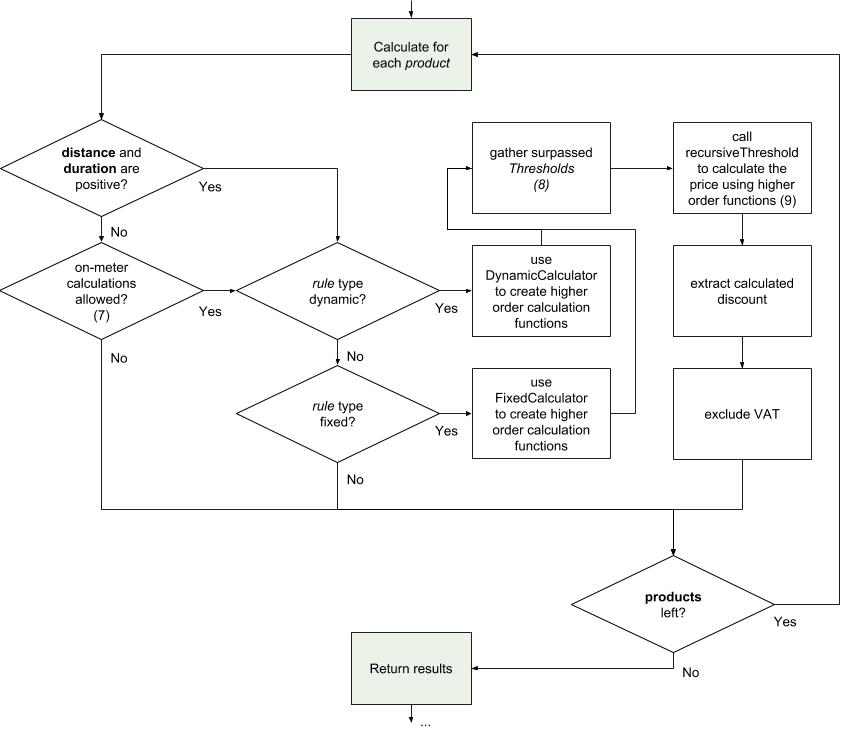
\includegraphics[width=1\textwidth]{Calculation}
	\caption[Calculation Flow]{The flow of a trip price calculation.}
	\label{fig:Calculation}
\end{figure}

When the user is authenticated, the system immediately requests the distance and duration of a ride by providing the departure and destination locations to the directions service. The directions service is provided to a Price class instantiation. The Price class waits for matched rules, upon which it will perform the price calculation. If all steps were succesfull, pricing rules were fetched for each requested product, discounts were either available or not, and the directions service is ready to provide the distance and duration of a ride.

%%%%%%%%%%%%%%%%%%%%%%%%%%%%%%%%%%%%%%%%%%%%%%%%%%%%%%%%%%%%%%%%%%%%%%%%%%%%%%%%
% Discounts %%%%%%%%%%%%%%%%%%%%%%%%%%%%%%%%%%%%%%%%%%%%%%%%%%%%%%%%%%%%%%%%%%%%%%%%%%%%%%%%
%
\subsection{Discounts}
The price calculation matches rules and discounts separately. Discounts were associated with rules in the legacy system, eliminating the amount of combinations of prices with or without discounts. A discount was either always active, or it was not. Having separation between the two enables users to define other locations and timeframes to both of them separately.

%%%%%%%%%%%%%%%%%%%%%%%%%%%%%%%%%%%%%%%%%%%%%%%%%%%%%%%%%%%%%%%%%%%%%%%%%%%%%%%%% Rules
%%%%%%%%%%%%%%%%%%%%%%%%%%%%%%%%%%%%%%%%%%%%%%%%%%%%%%%%%%%%%%%%%%%%%%%%%%%%%%%%
%
\subsection{Rules}
\mynote{Changes a lot, needs final version}
Rules and discounts are queried for each requested product as shown in step three and five of Figure \ref{fig:Calculation}. MongoDB’s aggregation framework allows documents to be aggregated in a multi-staged pipeline.

\subsubsection{Identification}
The first step in the pipeline matches all DaAppInstall entities with the identifiers sent along in the JWT payload: companyId and daAppInstallId.
\subsubsection{Links}
As shown in Figure \ref{fig:DataModel}, the DaAppInstall entities have multiple Links; ruleLinks and discountLinks. These links store data in a polymorphic hasManyThrough relation.
\subsubsection{Country}
Each company has a country, used to determine the default VAT and currency.
\subsubsection{Rules}
All documents are filtered based on geolocation and timeframes.
\subsubsection{Prices}
Prices are retrieved for each product that is associated with the matched rule. DynamicPrices and related thresholds, and FixedPrices and related thresholds.
\subsubsection{Sorting and Formatting}
The final step in the aggregate sorts and formats the results so that the Price class can calculate a price breakdown for each result.

%%%%%%%%%%%%%%%%%%%%%%%%%%%%%%%%%%%%%%%%%%%%%%%%%%%%%%%%%%%%%%%%%%%%%%%%%%%%%%%%
% Price Calculation Types
%%%%%%%%%%%%%%%%%%%%%%%%%%%%%%%%%%%%%%%%%%%%%%%%%%%%%%%%%%%%%%%%%%%%%%%%%%%%%%%%
% - What was proposed as a solution to store a week schedule in a database?
%
\section{Price Calculation Types}
Pricing information is validated before the calculation is started using the method shown in Listing \ref{lst:check-pricing-props}. The system should throw an error, as a price calculation can not proceed without the required information.

\begin{lstlisting}[caption={Find missing properties.}, label={lst:check-pricing-props}]
/**
 * Check if pricing contains valid properties and is not undefined.
 */
public static validPricingOrError(pricing: pricing | undefined): void {
	if (pricing === undefined) {
		throw new HttpError('Pricing data is undefined.');
	}
	const missing = [
		'prices',
		'rules',
		'country',
		'company',
		'type',
		'maxPassengers',
	].filter(prop => !(prop in pricing));
	if (missing.length) {
		throw new HttpError('Pricing data is missing properties:\n\t' + missing);
	}
}
\end{lstlisting}


Metrics are checked (distance duration)

Price calculator is picked depending on the rule type or if metrics are empty

\subsection{Dynamic}
The word dynamic in the dynamic price calculation means that the price can dynamically increase or decrease by a given values based on given parameters.
\subsection{Fixed}
The word fixed in the fixed price calculation means that a price is a given fixed amount under circumstances determined by the parameters.
\subsection{Meter}
The on-meter calculation simply returns a breakdown for which all values are zero. This is done by convention at taxiID, so that the mobile apps can calculate their own price based on a integrated meter inside the taxi.

%%%%%%%%%%%%%%%%%%%%%%%%%%%%%%%%%%%%%%%%%%%%%%%%%%%%%%%%%%%%%%%%%%%%%%%%%%%%%%%%
% Threshold Calculations
%%%%%%%%%%%%%%%%%%%%%%%%%%%%%%%%%%%%%%%%%%%%%%%%%%%%%%%%%%%%%%%%%%%%%%%%%%%%%%%%
%
\section{Threshold Calculations}
On top of each calculation type, prices can be defined after certain thresholds are surpassed. For example: if a taxi travels 25km, a threshold could be defined at 20km, after which the price will be 10 cents cheaper. In this case, the passenger pays a normal price for the 20 kilometers, and a cheaper price for the last 5 kilometers. The same holds for minute prices, but only for the dynamic price calculation. In the fixed price calculation, only kilometer thresholds can be defined. After a threshold is met, the fixed price will be replaced by a newly defined value. For any type of calculation, the algorithm works the same. Only the name of the metric used to measure thresholds and the actual calculation functions may change. For this reason, it is possible to define a function that recursively walks through all surpassed thresholds, then calculates a price using different calculations after each threshold was surpassed, as shown in Listing \ref{lst:threshold-recursion}

\begin{lstlisting}[caption={Recursive threshold calculation.}, label={lst:threshold-recursion}]
public static recursiveThreshold(
	thresholds: threshold[],
	calculation: Function,
	metric: number,
	cascaded: boolean = true,
): number {

	if (thresholds === undefined || thresholds.length < 1) {
		return calculation(undefined, metric);
	}

	if (!cascaded) {
		return calculation((<threshold>thresholds.shift()).value, metric);
	}

	const nextMetric = thresholds[0].threshold;
	const newMetric = metric - nextMetric;
	const price = calculation((<threshold>thresholds.shift()).value, newMetric);

	return price + Price.recursiveThreshold(
		thresholds,
		calculation,
		nextMetric,
	);
}
\end{lstlisting}

The Typescript type definitions reveal that calculation is of type Function, and thresholds is of type threshold[]. The base case returns the calculation with an undefined first argument. This forces the calculation method to use its default value, which is actually the normal kilometer or minute price. The base case will have the value of the first threshold that is met, assuring that the passenger pays the normal price up until that point. If the base case is not satisfied, the function checks whether the cascading boolean is true. This boolean determines whether each threshold should be evaluated, or only the last one. In case of the fixed price calculation, only the last threshold fixed price will be computed. But for the dynamic prices, each step has to be added to the total amount. Finally, the calculation is made using the next threshold,  and the recusive call is summed up with the calculated price. It is worth noting that even though this function is static and does not modify instance data, it is impure, leaving the passed thresholds array empty at the end.

%%%%%%%%%%%%%%%%%%%%%%%%%%%%%%%%%%%%%%%%%%%%%%%%%%%%%%%%%%%%%%%%%%%%%%%%%%%%%%%%
% Breakdown
%%%%%%%%%%%%%%%%%%%%%%%%%%%%%%%%%%%%%%%%%%%%%%%%%%%%%%%%%%%%%%%%%%%%%%%%%%%%%%%%
% - What should be included in the price breakdown?
% - VAT
% - Cents
%
\section{Breakdown}
The final result of the trip price calculation is a breakdown for every requested product. For example: if the mobile application requests prices for 'saloon' and 'limo' vehicle types, the response will at most contain an array with two breakdowns, for saloon and limo products. To ensure a seamless transition from the legacy price calculation system to TPS, the response formats should be identical. Still an improvement, if profitable enough, could be taken into consideration. One requirement of the price breakdown states that the tax should be included, but as shown in Listing \ref{lst:legacy-breakdown} the included tax is part of the breakdown. Is it by mistake or design?

\begin{lstlisting}[caption={Legacy price breakdown}, label={lst:legacy-breakdown}]
[
	{
		"vehicleType": "saloon",
		"maxPassengers": "4",
		"price": {
			"currency": "EUR",
			"total": 850,
			"breakdown": {
				"route": 802,
				"tax": 48,
				"toll": 0,
				"parking": 0,
				"waiting": 0,
				"discount": 0
			}
		},
		"fixedPrice": "true"
	}
]
\end{lstlisting}

Two possible solutions were proposed having VAT included in the price. The first solution extracts the tax element from the breakdown, so that the sum of the breakdown would add up to the total price where VAT is included in the price as shown in Listing \ref{lst:new-breakdown}. As demonstrated in Appendix \ref{appendix:slides_2_breakdown}, a breakdown is easily constructed in four steps when VAT is included.

\begin{lstlisting}[caption={Improved price breakdown}, label={lst:new-breakdown}]
[
	{
		"vehicleType": "estate",
		"maxPassengers": 4,
		"isEstimated": false,
		"price": {
			"breakdown": {
				"route": 8300,
				"toll": 0,
				"parking": 0,
				"waiting": 0,
				"discount": -1650
			},
			"currency": "EUR",
			"total": 6650,
			"tax": {
				"amount": 400,
				"percentage": 6
			}
		}
	},
	...
]
\end{lstlisting}

Keep in mind that unlike the listings the prices in the proposal are not displayed in cents. The second solution maintains the legacy format, but has to recalculate the prices without VAT. This could have downsides unlike the first approach:

\begin{enumerate}
	\item If an error is detected in the calculation, it is hard to trace back which components contributed to the total VAT. This would be even harder when each component uses its own VAT percentage.
	\item It takes extra steps to calculate the price of each component excluding VAT.
	\item Rounding the individual components could result in a sum that is not equal to the total displayed in the breakdown.
\end{enumerate}

The first proposal is chosen to be implemented, where the flag 'fixedPrice' is replaced by the 'isEstimated' flag to clearly reflect its purpose.

%%%%%%%%%%%%%%%%%%%%%%%%%%%%%%%%%%%%%%%%%%%%%%%%%%%%%%%%%%%%%%%%%%%%%%%%%%%%%%%%
% Conclusion
%%%%%%%%%%%%%%%%%%%%%%%%%%%%%%%%%%%%%%%%%%%%%%%%%%%%%%%%%%%%%%%%%%%%%%%%%%%%%%%%
%
\section{Conclusion}
\mynote{Conclusion for chapter 4}


% \item Which logic and information is required to calculate a trip price breakdown?
% 	      \begin{enumerate}[label*=\arabic*.]
% 		      % Timeframes, Locations, Vehicle types, priority, (broad view)
% 		      \item How are rules matched?
% 		            % VAT, rounding, discount, result breakdown, (all the parts explained)
% 		      \item Which parts of the system have an impact on the calculation result?
% 		            % Timeframes proposal
% 		      \item How should the concept of time schedules be realised?
% 	      \end{enumerate}